\section{Mechanizmy synchronizacji wątków – muteksy, zmienne warunkowe, bariery}

\subsection{Wprowadzenie} 
Zastosowanie obliczeń współbieżnych na ogół pozwala na osiągnięcie większej wydajności przetwarzania, w szczególności, gdy obliczenia są przeprowadzane na komputerach wieloprocesorowych. Pisanie poprawnie działających programów wielowątkowych wymaga specyfikacji i rozwiązania problemów, które w typowych obliczeniach sekwencyjnych nie występują. Problemy w~programowaniu współbieżnym biorą się z potrzeby synchronizowania wykonania wątków i zapewnienia im metod komunikowania się między sobą. Przy współbieżnym programowaniu należy zwrócić uwagę między innymi na następujące zagadnienia:

\begin{myitemize} 
\item Wyścigi -- do sytuacji wyścigu (ang. race condition) dochodzi wówczas, gdy dwa lub więcej procesów (wątków) wykonuje operacje na zasobach współdzielonych, a ostateczny wynik tej operacji w sposób przypadkowy zależy od czasu realizacji ciągów instrukcji.
\item Spójność danych (ang. data consistency) -- współpracujące wątki mogą jednocześnie odczytywać i zapisywać te same obszary pamięci. Dostęp do wspólnego zasobu musi być synchronizowany, w celu zapewnienia spójności danych, w przeciwnym przypadku, rezultat przetwarzania może być inny, niż oczekiwany. 
\end{myitemize} 

Rozwiązaniem wymienionych problemów jest zastosowanie synchronizacji, czyli kontroli przepływu sterowania pomiędzy wątkami (procesami), tak, żeby dopuszczalne były tylko ciągi instrukcji, które są zgodne z intencjami. System operacyjny czasu rzeczywistego QNX Neutrino dostarcza wielu metod synchronizacji pracy wątków. Jedne dostarczają jawnych metod synchronizacji, takich jak muteksy (mutex), zmienne warunkowe (conditional variables), bariery (barriers), zamki wstrzymujące (sleepon lock), zamki czytelników i pisarzy (reader writer lock), semafory (semaphores). Drugą grupę stanowią metody niejawne, które gwarantują synchronizację, poprzez wbudowane mechanizmy. Należą do nich szeregowanie FIFO (FIFO scheduling), wysyłanie komunikatów (messages), operacje atomowe (atomic operations). Oprócz barier i blokad wstrzymujących wszystkie przytoczone mechanizmy pozwalają synchronizować nie tylko wątki, ale również procesy. Dodatkowym aspektem, który może mieć znaczenie jest możliwość synchronizacji wątków (procesów) w sieci. Spośród wymienionych metod semafory (nazwane) oraz komunikaty spełniają to wymaganie. 
W trakcie laboratorium omówimy podstawowe operacje synchronizacji wątków (muteksy, zmienne warunkowe, bariery) oraz pojęcia z nimi związane (wzajemne wykluczanie, sekcja krytyczna, zakleszczenia, inwersja priorytetów). Rozważania będą ilustrowane przykładami pracy programów współbieżnych z zastosowaniem mechanizmów synchronizacji pracy wątków.  

\subsection{Wyścigi} 

Scenariusz, w którym występuje wyścig o współdzielony zasób przedstawia przykład. Wątek główny (wątek 1) wykonuje się współbieżnie z wątkiem 2. Oba wątki współdzielą zmienną \lstinline[style=MyCStyle]{b}. Problem pojawia się w sytuacji, gdy dwa wątki próbują ''jednocześnie'' zmodyfikować dane. W rezultacie wynik operacji będzie nieprzewidywalny i zależny od kolejności wykonania ciągów instrukcji przez poszczególne wątki. Jeden ze scenariuszy przedstawiono na rysunku~\ref{fig:race}.  


\begin{figure}[!h]
\centering
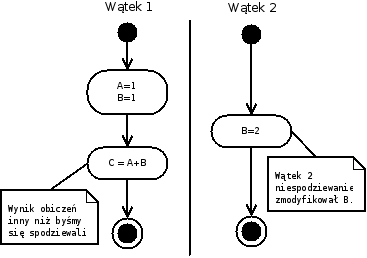
\includegraphics[width=0.5\textwidth]{img/thrd_race}
\caption{Ilustracja wyścigu (race condition) pomiędzy dwoma wątkami}
\label{fig:race}
\end{figure}

\begin{example}{[Brak synchronizacji pracy wątków]} \label{ex:nosynchro}
Skompilować, uruchomić kilkakrotnie program oraz zaobserwować różne scenariusze wykonania programu w~zależności od czasu pracy poszczególnych wątków.  

\lstinputlisting[caption=Ilustracja braku synchronizacji pracy wątków,style=MyCStyle,label=src:racecond]{src/lab6/racecond.c}
\end{example}

\subsection{Muteksy}

Popularną i ogólną metodą synchronizowania pracy wątków jest zapewnienie dostępu do współdzielonych zasobów (np. pamięci) tylko dla jednego z potencjalnie wielu wykonywanych wątków lub procesów. Wymaganie to nazywa się wzajemnym wykluczaniem (ang. mutual exclusion). System QNX RTOS dostarcza zgodnego ze standardem POSIX mechanizmu wzajemnego wykluczania zwanego muteksem, który jest specjalną formą bardziej ogólnego mechanizmu semafora. Muteks jest rodzajem blokady, którą może zająć tylko jeden wątek jednocześnie. Jeśli jeden wątek zajął muteks i drugi w tym czasie próbuje zająć muteks, to będzie on w stanie zablokowanym (ang. locked). Muteks może być zwolniony tylko przez ten wątek, który go zajął. W tej sytuacji, wątek drugi jest w stanie odblokowanym (ang. unlocked). System operacyjny gwarantuje, że nie pojawią się wyścigi pomiędzy wątkami o zajęcie muteksu. Tylko jeden wątek może zająć muteks, pozostałe będą zablokowane. Ciąg instrukcji, który jest wykonywany tylko przez jeden, z potencjalnie wielu wątków (procesów) nazywamy \underline{sekcją krytyczną} (ang. critical section). Zasadę działania muteksu, w przypadku dwóch wątków, pracujących współbieżnie przedstawia rysunek~\ref{fig:mutex}. 

\begin{figure}[!h]
\centering
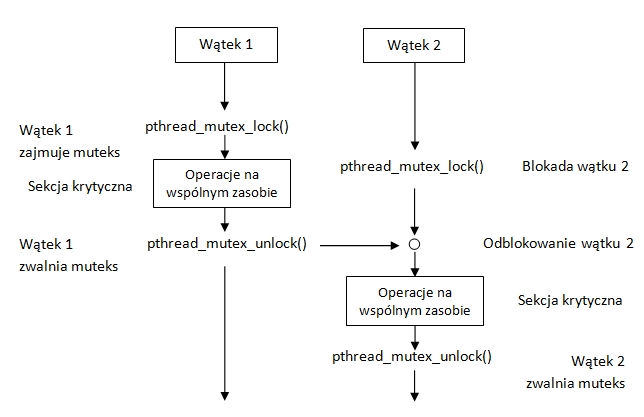
\includegraphics[width=0.85\textwidth]{img/mutex}
\caption{Zasada działania muteksów}
\label{fig:mutex}
\end{figure}

Typowy sposób użycia muteksu składa się z następujących operacji: 

\begin{myenumerate} 
\item Utworzenie muteksu (zmiennej typu \lstinline[style=MyCStyle]{pthread_mutex_t}) i~inicjalizacja.
\item Kilka wątków próbuje zająć muteks, tylko jednemu się udaje. 
\item Wykonanie operacji na zasobie w sekcji krytycznej, przez wątek, który zajął muteks. 
\item Zwolnienie muteksu.
\item Zajęcie muteksu i powtórzenie procesu.
\item Skasowanie muteksu.
\end{myenumerate} 

\subsubsection{Tworzenie i kasowanie muteksów}

Muteks jest reprezentowany w programie za pomocą zmiennej \lstinline[style=MyCStyle]{pthread_mutex_t}. Funkcja \lstinline[style=MyCStyle]{pthread_mutex_init()} służy do inicjalizacji tego obiektu:

\begin{lstlisting}[style=MyCStyle]
pthread_mutex_t mutex = PTHREAD_MUTEX_INITIALIZER;

int pthread_mutex_init(
            pthread_mutex_t* mutex,
            const pthread_mutexattr_t* attr );
\end{lstlisting}


gdzie 
\begin{myitemize}
\item \lstinline[style=MyCStyle]{mutex} -- jest wskaźnikiem do obiektu, który chcemy zainicjalizować. 
\item \lstinline[style=MyCStyle]{attr} -- jest albo NULL (atrybuty domyślne) albo wskaźnikiem do struktury definiującej atrybuty muteksu.  
\end{myitemize}

Muteksy możemy inicjalizować nie tylko dynamicznie, używając struktury \lstinline[style=MyCStyle]{attr}, ale również  statycznie, poprzez zastosowanie makra \lstinline[style=MyCStyle]{PTHREAD_MUTEX_INITIALIZER}, które zapewnia przypisanie domyślnych wartości do muteksu. Domyślnie muteks jest w stanie odblokowanym. 
Do kasowania muteksu służy funkcja:

\begin{lstlisting}[style=MyCStyle]
int pthread_mutex_destroy( pthread_mutex_t* mutex );
\end{lstlisting}

Funkcja \lstinline[style=MyCStyle]{pthread_mutex_destroy()} kasuje zasoby zajęte przez muteks. Kasowany muteks powinien być w stanie odblokowanym. Zajęty muteks może być skasowany przez właściciela muteksu. W takim przypadku wątki czekające na muteksie zostają odblokowane. 

\subsubsection{Zajmowanie i zwalnianie muteksów}

Funkcja  \lstinline[style=MyCStyle]{pthread_mutex_lock()} służy do zajęcia muteksu przez wątek. Jeśli muteks jest zajęty przez inny wątek, to pozostałe będą w stanie zablokowanym, aż do momentu, gdy muteks zostanie odblokowany. Gdy muteks jest wolny, to następuje jego zajęcie przez wątek bieżący.

\begin{lstlisting}[style=MyCStyle]
int pthread_mutex_lock( pthread_mutex_t* mutex );
\end{lstlisting}

gdzie mutex jest wskaźnikiem do obiektu typu \lstinline[style=MyCStyle]{pthread_mutex_t}. Zablokowane wątki mogą czekać dowolnie długo na odblokowanie muteksu. Funkcją, która umożliwia zajęcie muteksu na określony czas jest funkcja o~sygnaturze:

\begin{lstlisting}[style=MyCStyle]
int pthread_mutex_timedlock( 
                  pthread_mutex_t * mutex,
                  const struct timespec * abs_timeout );
\end{lstlisting}

gdzie \lstinline[style=MyCStyle]{mutex} jest wskaźnikiem do obiektu typu \lstinline[style=MyCStyle]{pthread_mutex_t}, \lstinline[style=MyCStyle]{abs_timeout} wskaźnikiem do struktury:

\begin{lstlisting}[style=MyCStyle]
struct timespec {
   time_t   tv_sec;
   long     tv_nsec;
}
\end{lstlisting}

opisującej maksymalny czas, do którego ma czekać wątek, w celu odblokowania muteksu (czas absolutny). 
Używanie funkcji \lstinline[style=MyCStyle]{pthread_mutex_lock()}, czy \lstinline[style=MyCStyle]{pthread_mutex_timedlock()} do zajęcia muteksu powoduje zablokowanie wątków wywołujących, gdy muteks jest zajęty. Na ogół taki stan jest pożądany. Zdarzają się jednak sytuacje, kiedy wątek zamiast czekać na zwolnienie muteksu, może wykonać użyteczne operacje. Biblioteka pthread dostarcza użytecznego mechanizmu \lstinline[style=MyCStyle]{pthread_mutex_trylock()}, który jest formą nieblokującego zajęcia muteksu.

\begin{lstlisting}[style=MyCStyle]
int pthread_mutex_trylock( pthread_mutex_t* mutex );
\end{lstlisting}

Funkcja \lstinline[style=MyCStyle]{pthread_mutex_trylock()} próbuje zająć muteks, ale nie blokuje wątków wywołujących, gdy muteks jest zajęty. Należy pamiętać, że aby odblokowywać muteks wówczas, kiedy funkcja \lstinline[style=MyCStyle]{pthread_mutex_trylock} zwróci kod sukcesu. Funkcja ta jest użyteczna, w przypadku zakleszczeń i sytuacji związanych z inwersją priorytetów. Funkcją, która pozwala na zwolnienie muteksu jest \lstinline[style=MyCStyle]{pthread_mutex_unlock()}:

\begin{lstlisting}[style=MyCStyle]
int pthread_mutex_unlock( pthread_mutex_t* mutex );
\end{lstlisting}

Funkcja \lstinline[style=MyCStyle]{pthread_mutex_unlock()} zwalnia muteks. Gdy istnieją wątki, które są zablokowane na muteksie, to zostaje odblokowany wątek, z najwyższym priorytetem i on staje się właścicielem muteksu. Gdy brak wątków zajmujących muteks, to stan muteksu zostaje ustawiony na wolny. 

\begin{figure}[!h]
\centering
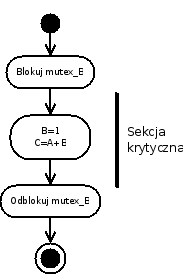
\includegraphics[width=0.3\textwidth]{img/thrd_mutex}
\caption{Przykład użycia muteksów}
\label{fig:mutex}
\end{figure}

\begin{example}{[Synchronizacja pracy wątków]}
Przykład jest modyfikacją przykładu~\ref{ex:nosynchro} i~pokazuje sposób użycia muteksu do ochrony wspólnych zasobów. Skompilować, uruchomić program oraz prześledzić jego działanie. 

\lstinputlisting[caption=Przykład użycia muteksów,style=MyCStyle,label=src:mutex]{src/lab6/mutex.c}
\end{example}

\subsubsection{Problemy przy stosowaniu muteksów}

\textbf{Zakleszczenia}. Czasami użycie jednego muteksu do ochrony wspólnych danych jest niewystarczające. W przypadku jednoczesnego stosowania więcej niż jednego muteksu pojawiają się problemy, które nie występują, gdy stosujemy jeden muteks. Jednym z nich jest zakleszczenie (ang. deadlock), czyli sytuacja, gdy dwa (lub więcej wątków) czekają na siebie nawzajem, zajmując muteks (zasób) i jednocześnie czekają na zwolnienie innego muteksu (zasobu), zajętego przez inne wątki, potrzebnego do kontynuacji swojego działania. Klasyczną sytuacją jest scenariusz przedstawiony na rysunku~\ref{fig:deadlock}. 

\begin{figure}[!h]
\centering
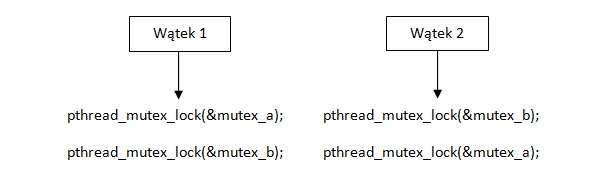
\includegraphics[width=0.8\textwidth]{img/deadlock}
\caption{Sytuacja zakleszczenia wątków (deadlock)}
\label{fig:deadlock}
\end{figure}

Oba wątki mogą ukończyć pierwszy etap scenariusza (zablokowanie na muteksach  \lstinline[style=MyCStyle]{mutex_a} oraz  \lstinline[style=MyCStyle]{mutex_b}) orientacyjnie w tym samym czasie. Jeśli ciąg instrukcji będzie taki, że np. wątek 2 najpierw zablokuje  \lstinline[style=MyCStyle]{mutex_b}, to wątek 1 zostanie zablokowany na muteksie, który jest już zajęty przez wątek 2, a następnie dojdzie do zablokowania wątku 2. Istnieją dwa typowe rozwiązania tego problemu:

\begin{myitemize}
\item Zajmowanie muteksów w ściśle określonej kolejności. (np. najpierw \lstinline[style=MyCStyle]{mutex_a}, a później \lstinline[style=MyCStyle]{muteks_b}).
\item Zastosowanie nieblokującej funkcji do zajmowania muteksu. Po zablokowaniu np. \lstinline[style=MyCStyle]{mutex_a}, używamy nieblokującej funkcji \lstinline[style=MyCStyle]{pthread_mutex_trylock()}, aby sprawdzić, czy \lstinline[style=MyCStyle]{mutex_b} jest zajęty; jeśli tak, to zwalniamy \lstinline[style=MyCStyle]{mutex_a} i~\lstinline[style=MyCStyle]{mutex_b} i powtarzamy całą procedurę.
\end{myitemize}

\begin{example}{[Zakleszczenie wątków]}
Przykład pokazuje zakleszczenie wątków, w przypadku, gdy zmienna \lstinline[style=MyCStyle]{asynchron = 0}. Ponadto pokazano metodę rozwiązania problemu zakleszczenia poprzez zastosowanie nieblokującej próby zajęcia muteksu, w przypadku, gdy zmienna  \lstinline[style=MyCStyle]{asynchron = 1}. Uruchomić program z dwiema opcjami i~zbadać jego zachowanie. 

\lstinputlisting[caption=Deadlock,style=MyCStyle,label=src:asynchron]{src/lab6/asynchron.c}
\end{example}

\textbf{Inwersja priorytetów}. Inwersja priorytetów jest problemem, który pojawia się w sytuacji, gdy występują conajmniej trzy wątki o różnych priorytetach. Istnieje wtedy konflikt pomiędzy wymaganiami nakładanymi przez metody synchronizacji (np. muteksy), a wymaganiami, dotyczącymi szeregowania wątków. Wykonywany jest wątek o niższym priorytecie, w sytuacji, gdy wątek o wyższym priorytecie został zablokowany na operacji synchronizacyjnej. 

Przypuśćmy, że wątek 1, o najniższym priorytecie zajął muteks. Wątek 3, o najwyższym priorytecie, używa wspólnego zasobu z wątkiem 1 i próbuje zająć ten sam muteks poprzez wywołanie funkcji \lstinline[style=MyCStyle]{pthread_mutex_lock()}. Operacja nie udaje się i wątek 3 zostaje zablokowany na operacji synchronizacyjnej, mimo, iż ma wyższy priorytet, niż wątek 1. Jeśli pojawi się wątek 2 (np. na skutek aktywności innych wątków), o pośrednim priorytecie i wywłaszczy wątek 1, to wątek 1 nie będzie mógł zwolnić muteksu. Wówczas, wątek 3 będzie zablokowany na operacji synchronizacyjnej, a wątek 2 będzie się wykonywał, mimo, iż ma mniejszy priorytet, niż wątek 3. 

W systemie QNX Neutrino są stosowane dwie strategie zapobiegania inwersji priorytetów: 
\begin{myenumerate}
\item Dziedziczenie priorytetów polega na tymczasowym zwiększeniu priorytetu wątku, który posiada zasób (muteks) do najwyższego priorytetu wątku, który ubiega się o zasób. Priorytet wątku posiadającego zasób zostanie przywrócony do pierwotnego, po jego zwolnieniu. Schemat ten zapewnia, że wątki o najwyższych priorytetach będą zablokowane na najkrótszy możliwy czas, jednocześnie rozwiązując problem inwersji priorytetów. 
\item Zastosowanie protokołu wykorzystującego pułap priorytetów -- polega na przydzieleniu zasobowi (muteksowi) priorytetu statycznego, większego od najwyższego priorytetu wątków, które o dany zasób będą konkurowały. Gdy jakiś wątek będzie próbował zająć zasób, to zostanie mu przydzielony tymczasowo priorytet związany z zasobem. Po zwolnieniu zasobu priorytet wątku wraca do wartości pierwotnej. 
\end{myenumerate}

\subsection{Zmienne warunkowe} 

\subsubsection{Wstęp}

Zmienne warunkowe dostarczają alternatywnego sposobu synchronizacji wątków. Podczas gdy muteksy synchronizują dostęp poszczególnych wątków do danych, zmienne warunkowe umożliwiają wątkom uzyskiwać informację (sygnalizować) o aktualnym stanie współdzielonych zasobów. Bez mechanizmu sygnalizowania zmiennych warunkowych, jeden z wątków musiałby nieustannie badać w pętli (potencjalnie w sekcji krytycznej) spełnienie pewnego warunku. Taki zabieg prowadziłby do niekorzystnego zużycia czasu procesora. Zmienna warunkowa pozwala osiągnąć ten sam cel bez użycia nieskończonej pętli. 
Zmienna warunkowa jest mechanizmem sygnalizowania informacji i powinna być skojarzona z muteksem, który z kolei chroni dostępu do wspólnego zasobu (danych). Trzy podstawowe operacje dokonywane na zmiennych są następujące: 

\begin{myitemize}
\item Oczekiwanie na zmienną warunkową (wait) – zwalnia muteks i zawiesza wątek aż do momentu zasygnalizowania zmiennej warunkowej.
\item Sygnalizowanie zmiennej warunkowej (signal) – sygnalizuje zmienną warunkową i wznawia zawieszony wątek.
\item Sygnalizowanie zmiennej warunkową (broadcast) – sygnalizuje zmienną warunkową i wznawia wszystkie wątki zawieszone w kolejce zmiennej warunkowej. 
\end{myitemize} 

Typowy scenariusz synchronizacji zmiennymi warunkowymi jest następujący: 
\begin{myitemize}
\item Zadeklarować i zainicjalizować zmienną warunkową.
\item Zadeklarować i zainicjalizować stowarzyszony ze zmienną warunkową muteks.
\item Zablokować muteks stowarzyszony ze zmienną warunkową.
\item Kilka wątków zostaje zawieszonych w kolejce na zmiennej warunkowej i oczekują aż jakiś inny wątek zasygnalizuje sytuację sprzyjającą dalszej pracy. 
\item Sygnalizacja zmiennej warunkowej. 
\item Jeden z zawieszonych wątków (pierwszy w kolejce) wznawia swoje działanie. Pozostałe wątki oczekują nadal nad zmienną warunkową, aż do kolejnego zasygnalizowania zmiennej.
\item Odblokować muteks stowarzyszony ze zmienną warunkową.
\item Skasowanie muteksu.
\item Skasowanie zmiennej warunkowej.
\end{myitemize}


\subsubsection{Tworzenie i kasowanie zmiennych warunkowych}

Zmienna warunkowa jest reprezentowana w programie, jako zmienna typu \lstinline[style=MyCStyle]{pthread_cond_t} i musi być zainicjalizowana przed użyciem. Podobnie jak w przypadku muteksów istnieją dwa sposoby inicjalizacji statycznie, bądź dynamicznie. 
\lstinline[style=MyCStyle]{pthread_cond_t cond = PTHREAD_COND_INITIALIZER;}

\begin{lstlisting}[style=MyCStyle]
int pthread_cond_init( pthread_cond_t* cond,
                       pthread_condattr_t* attr );
\end{lstlisting}

gdzie 

\begin{myitemize}
\item \lstinline[style=MyCStyle]{cond} -- jest wskaźnikiem do zmiennej warunkowej \lstinline[style=MyCStyle]{pthread_cond_t}.
\item \lstinline[style=MyCStyle]{attr} -- jest albo \lstinline[style=MyCStyle]{NULL} (atrybuty domyślne) albo wskaźnikiem do struktury definiującej atrybuty muteksu.  
\end{myitemize}


Zmienne warunkowe możemy inicjalizować nie tylko dynamicznie, używając struktury \lstinline[style=MyCStyle]{attr}, ale również  statycznie, poprzez zastosowanie makra \lstinline[style=MyCStyle]{PTHREAD_COND_INITIALIZER}, które zapewnia przypisanie domyślnych wartości do zmiennej warunkowej. Do kasowania zmiennej warunkowej służy funkcja:


\begin{lstlisting}[style=MyCStyle]
int pthread_cond_destroy( pthread_cond_t* cond );
\end{lstlisting}

Funkcja \lstinline[style=MyCStyle]{pthread_cond_destroy} kasuje zasoby zajęte przez zmienną warunkową.

\subsubsection{Czekanie i sygnalizowanie zmiennej warunkowej}

Funkcja \lstinline[style=MyCStyle]{pthread_cond_wait()} pozwala na oczekiwanie na zmienną warunkową:

\begin{lstlisting}[style=MyCStyle]
int pthread_cond_wait( pthread_cond_t* cond,
                       pthread_mutex_t* mutex );
\end{lstlisting}

gdzie 

\begin{myitemize}
\item \lstinline[style=MyCStyle]{cond} -- jest wskaźnikiem do zmiennej warunkowej \lstinline[style=MyCStyle]{pthread_cond_t}.
\item \lstinline[style=MyCStyle]{mutex} -- stowarzyszony muteks. 
\end{myitemize}

Funkcja \lstinline[style=MyCStyle]{pthread_cond_wait()} zawiesza wątek na zmiennej warunkowej \lstinline[style=MyCStyle]{cond}, ustawia go w kolejce wątków oczekujących i jednocześnie odblokowuje stowarzyszony muteks. Funkcja ta powinna być wywołana, wówczas kiedy muteks jest zajęty i automatycznie ponownie zamknie muteks po wyjściu z funkcji. 

Istnieje odmiana funkcji, która pozwala czekać na zmiennej warunkowej przez określony czas:

\begin{lstlisting}[style=MyCStyle]
int pthread_cond_timedwait(
            pthread_cond_t* cond,
            pthread_mutex_t* mutex,
            const struct timespec* abstime );
\end{lstlisting}

gdzie 
\begin{myitemize}
\item \lstinline[style=MyCStyle]{abstime} -- jest wskaźnikiem do struktury \lstinline[style=MyCStyle]{timespec}, która definiuje maksymalny absolutny czas blokowania wątku.
\end{myitemize}

Wątek w przypadku funkcji \lstinline[style=MyCStyle]{pthread_cond_wait()} lub \lstinline[style=MyCStyle]{pthread_cond_timedwait()} jest zablokowany do czasu zasygnalizowania zmiennej warunkowej przez  inny z wątków przez funkcję: 

\begin{lstlisting}[style=MyCStyle]
int pthread_cond_signal( pthread_cond_t* cond );
\end{lstlisting}

Funkcja odblokowuje wątek o najwyższym priorytecie, który czeka na zmiennej warunkowej \lstinline[style=MyCStyle]{cond}. Gdy wątków o najwyższym priorytecie jest więcej, odblokowany będzie ten, który czeka najdłużej. Odblokowanie wszystkich wątków, które czekają na zmiennej warunkowej można zrealizować poprzez wywołanie funkcji: 

\begin{lstlisting}[style=MyCStyle]
int pthread_cond_broadcast( pthread_cond_t* cond );
\end{lstlisting}

Wątki są odblokowane w zależności od wysokości priorytetów. W przypadku, gdy istnieje kilka wątków, o takich samych priorytetach, to wątki będą odblokowywane wg strategii FIFO. Działanie zmiennej warunkowej przedstawiono na rysunku~\ref{fig:condvar}. 

\begin{figure}[!h]
\centering
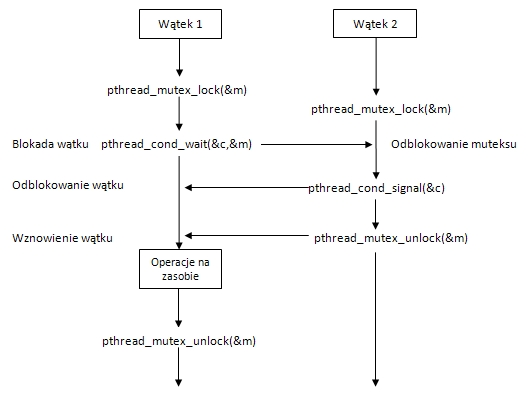
\includegraphics[width=0.75\textwidth]{img/condvar}
\caption{Idea działania zmiennej warunkowej}
\label{fig:condvar}
\end{figure}

\begin{example}{[Zmienne warunkowe]}
Program tworzy trzy wątki. Wątek główny pracuje jako zarządca (manager) i co 2 sekundy deleguje do pracy jeden z dwóch wątków wykonawczych. Realizacja zadania zajmuje każdemu z wątków wykonawców 3 sekundy. Skompilować program, uruchomić i prześledzić jego współbieżną pracę.
\lstinputlisting[caption=Zastosowanie zmiennej warunkowej,style=MyCStyle,label=src:condvar]{src/lab6/condvar.c}
\end{example}

\subsection{Bariery} 

\subsubsection{Tworzenie i kasowanie bariery} 

Synchronizacja przy użyciu bariery umożliwia koordynację pracy algorytmów. Bariera definiuje punkt w programie, do którego muszą dotrzeć wszystkie wątki zanim rozpoczną dalsze wykonanie. Liczba wątków potrzebnych do przełamania bariery jest definiowana w chwili tworzenia bariery.

\begin{figure}[!h]
\centering
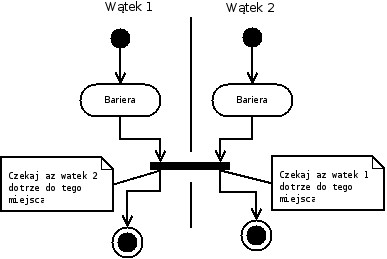
\includegraphics[width=0.5\textwidth]{img/thrd_barrier}
\caption{Idea działania bariery}
\label{fig:thrd_barrier}
\end{figure}

Bariera jest reprezentowana w programie, jako zmienna typu \lstinline[style=MyCStyle]{pthread_barrier_t} i musi być zainicjalizowana przed użyciem. Inicjalizacja bariery odbywa się poprzez wywołanie następującej funkcji: 

\begin{lstlisting}[style=MyCStyle]
int pthread_barrier_init( 
                    pthread_barrier_t * barrier,
                    const pthread_barrierattr_t * attr
                    unsigned int count );

\end{lstlisting}

gdzie 

\begin{myitemize}
\item \lstinline[style=MyCStyle]{barrier} -- wskaźnik do obiektu typu \lstinline[style=MyCStyle]{pthread_barrier_t}, który chcemy zainicjalizować. 
\item \lstinline[style=MyCStyle]{attr} -- jest albo \lstinline[style=MyCStyle]{NULL} (atrybuty domyślne) albo wskaźnikiem do struktury definiującej atrybuty bariery \lstinline[style=MyCStyle]{pthread_barrierattr_t}.
\item \lstinline[style=MyCStyle]{count} -- liczba wątków, które muszą dojść do momentu wywołania funkcji \lstinline[style=MyCStyle]{pthread_barrier_wait()}, aby wszystkie mogły kontynuować dalej swoje działanie. 
\end{myitemize}

Bariery możemy inicjalizować nie tylko dynamicznie, używając struktury attr, ale również  statycznie, poprzez zastosowanie makra \lstinline[style=MyCStyle]{PTHREAD_BARRIER_INITIALIZER(count)}, które zapewnia przypisanie domyślnych wartości do bariery oraz liczby \lstinline[style=MyCStyle]{count}, omówionej poprzednio.

Do kasowania bariery służy funkcja:

\begin{lstlisting}[style=MyCStyle]
int pthread_barrier_destroy(
       pthread_barrier_t * barrier );
\end{lstlisting}

Funkcja \lstinline[style=MyCStyle]{pthread_barrier_destroy()} kasuje zasoby zajęte przez barierę. 

\subsubsection{Czekanie na barierze}

Funkcja  \lstinline[style=MyCStyle]{pthread_barrier_wait()} pozwala na synchronizację wątków na barierze: 

\begin{lstlisting}[style=MyCStyle]
	int pthread_barrier_wait( pthread_barrier_t * barrier );
\end{lstlisting}

Wątki, które wywołują funkcję są blokowane, aż do momentu, gdy wymagana liczba wątków (\lstinline[style=MyCStyle]{count}) wywołała funkcję \lstinline[style=MyCStyle]{pthread_barrier_wait()}, wówczas bariera jest przełamywana, jednemu z wątków (nieokreślonemu) jest zwracana wartość \lstinline[style=MyCStyle]{BARRIER_SERIAL_THREAD}, natomiast innym jest zwracana wartość zero. Po tym etapie stan bariery jest ustawiany do wartości po wywołaniu inicjalizacji bariery. 

\begin{example}{[Brak synchronizacji]}
Program zawiera dwa wątki. Wątek 1 oblicza pewną wartość $a$, wątek 2 oblicza wartość $b$. Następnie wątek 1 powinien obliczyć $c=a+b$, a wątek 2 powinien obliczyć $d=a\cdot b$ -- zobacz rysunek~\ref{fig:thrd_async_example}. Przykład ilustruje brak synchronizacji pracy wątków.

\begin{figure}[!h]
\centering
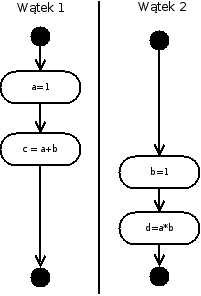
\includegraphics[width=0.35\textwidth]{img/thrd_async_example}
\caption{Idea działania bariery}
\label{fig:thrd_async_example}
\end{figure}

\lstinputlisting[caption=Brak synchronizacji pracy wątków,style=MyCStyle,label=src:nosynchro]{src/lab6/nosynchro.c}
\end{example}

\begin{example}{[Użycie bariery]} Poniższy przykład jest modyfikacją poprzedniego. Obliczenia zsynchronizowano używając bariery -- zobacz rysunek~\ref{fig:thrd_barrier_example}. 

\begin{figure}[!h]
\centering
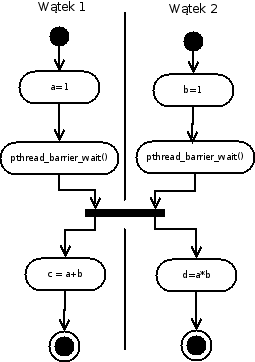
\includegraphics[width=0.35\textwidth]{img/thrd_barrier_example}
\caption{Idea działania bariery}
\label{fig:thrd_barrier_example}
\end{figure}

\lstinputlisting[caption=Brak synchronizacji pracy wątków,style=MyCStyle,label=src:synchrobarrier]{src/lab6/synchrobarrier.c}

\end{example}

\subsection{Ćwiczenia}
 
\begin{myenumerate}
\item Zaproponować współbieżną (równoległą – gdy dysponujemy komputerem wieloprocesorowym) wersję programu do obliczania liczby $\pi$ za pomocą wątków i mechanizmów synchronizacji. Matematycznie wiadomo, że:

\begin{equation}\nonumber 
\displaystyle\int_0^1{\frac{4}{1+x^2}dx}=\pi
\end{equation}

Całkę oznaczoną możemy aproksymować jako sumę:

\begin{equation}\nonumber 
\sum_{i=0}^N\frac{4}{1+x_i^2}\Delta x\approx\pi
\end{equation}

Ilustrację graficzną aproksymacji liczby $\pi$ można znaleźć na rysunku~\ref{fig:piApprox}. Należy zadeklarować sumę, jak zmienną globalną oraz obliczać ją w sekcji krytycznej. Synchronizację dostępu do zmiennej globalnej zapewnić poprzez zastosowanie muteksów.

\begin{figure}[!h]
\centering
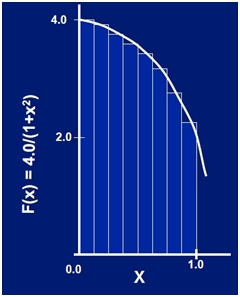
\includegraphics[width=0.4\textwidth]{img/piApprox}
\caption{Idea aproksymacji liczby $\pi$}
\label{fig:piApprox}
\end{figure}

\lstinputlisting[caption=Kod źródłowy sekwencyjnej wersji do obliczania liczby $\pi$,style=MyCStyle,label=src:piApprox]{src/lab6/piApprox.c}

\item Należy przeczytać tekst dot. inwersji prioryterów w~oprogramowaniu sondy marsjańskiej Pathfinder  \href{http://research.microsoft.com/en-us/um/people/mbj/mars\_pathfinder/Mars\_Pathfinder.html}{http://research.microsoft.com/en-us/um/people/mbj/mars\_pathfinder/Mars\_Pathfinder.html}.
\end{myenumerate}

\cleardoublepage
